% Created with jtex v.1.0.17
\documentclass{article}
\PassOptionsToPackage{short, nodayofweek}{datetime}


% Start Curvenote Definitions

% Pass Options Section
% base
\PassOptionsToPackage{normalem}{ulem}
\PassOptionsToPackage{utf8}{inputenc}

% template
\PassOptionsToPackage{framemethod=TikZ}{mdframed}
\PassOptionsToPackage{x11names, svgnames}{xcolor}

%%% PACKAGES

% base
\usepackage{inputenc}
\usepackage{url}
\usepackage{graphicx}
\usepackage{adjustbox}
\usepackage{amssymb}
\usepackage{amsfonts}
\usepackage{amsmath}
\usepackage{enumitem}
\usepackage{nicefrac}
\usepackage{booktabs}
\usepackage{microtype}
\usepackage{hyperref}
\usepackage{ulem}
\usepackage{enumitem}
\usepackage{float}
\usepackage{datetime}
\usepackage{xkeyval}
\usepackage{framed}
\usepackage{doi}

% template
\usepackage{natbib}
\usepackage{fancyvrb}
\usepackage{mdframed}
\usepackage{xcolor}

%%%


%%%% Setup Section

% base
\graphicspath{{.}}
% template
\sloppy
\newenvironment{aside}{\begin{framed}}{\end{framed}}
\newmdenv[linewidth=2pt,linecolor=CornflowerBlue,topline=false,bottomline=false,rightline=false,leftline=true,skipabove=20,skipbelow=20,leftmargin=20,rightmargin=20]{callout}
\newfloat{code}{thp}{loc}
\floatname{code}{Program}
\raggedbottom
\bibliographystyle{abbrvnat}
\setcitestyle{authoryear,open={(},close={)},semicolon,aysep={,}}

% End Curvenote Definitions




% colors for hyperlinks
\hypersetup{colorlinks=true, allcolors=blue}
\hypersetup{
pdftitle={\@title},
pdfsubject={},
pdfauthor={\@author},
pdfkeywords={},
addtopdfcreator={Written in Curvenote}
}

\usepackage{curvenote}

\title{Scenario 0}

\newdate{articleDate}{21}{4}{2024}
\date{\displaydate{articleDate}}

\author{\bfseries Hector Nieto\mdseries\\ICA-CSIC\\\AND\bfseries Benjamin Mary\mdseries\\ICA-CSIC\\\AND\bfseries Vicente Burchard-Levine\mdseries\\ICA-CSIC\\}

\begin{document}

\maketitle
\keywords{DA}

\begin{figure}[!htbp]
\centering
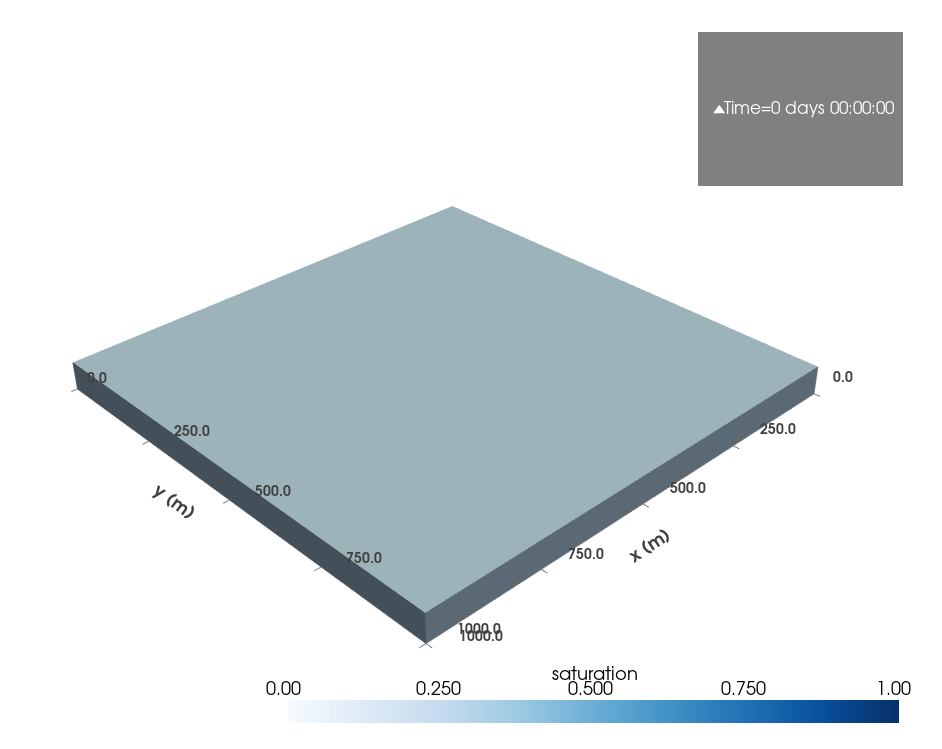
\includegraphics[width=0.75\linewidth]{files/EOMAJI_mesh-509781dd4b086cb32383299dabc9f88d.png}
\caption*{EO-MAJI-IrrDelineation}
\end{figure}

\section{Model}

\begin{itemize}
\item The \textbf{regional domain size} is 1000x1000m square, flat. \textbf{Irrigation local size} is a 100x100m square centered on the regional domain.
\end{itemize}

\textbf{Soil and Vegetation}

\begin{itemize}
\item The vegetation is uniform on all the regional domain size, with \textbf{root depth} of 1m typical from herbaceous crop.
\item The soil is homogeneous all over the regional domain.
\item \textbf{At time 0}, the soil is dry with an initial pressure head of -30m that is equivalent to a saturation level of 0.3?.
\end{itemize}

\textbf{Atmospheric Boundary conditions}

\begin{itemize}
\item The irrigation consist in a single event at ?? sec (day ??).
\item The irrigation rate is \textbf{5e-07} m/s during \textbf{21600} sec. This is equivalent to 43.2 mm/day during 6hours.
\item The \textbf{potential ETp} is homogeneous all over the domain and with time, set to -1e-07 m/s.
\item \textbf{No flow} boundary conditions are imposed outside the regional domain.
\end{itemize}

\textbf{Observations}

\begin{itemize}
\item Earth Observations are available at a \textbf{daily frequency}.
\end{itemize}

\begin{figure}[!htbp]
\centering
\includegraphics[width=0.75\linewidth]{files/vtksaturation-6351a4b146f09c4ae6b6fcd05adccf86.gif}
\caption*{Saturation over the course of the irrigation}
\end{figure}

\section{Irrigation delimitation}

\begin{figure}[!htbp]
\centering
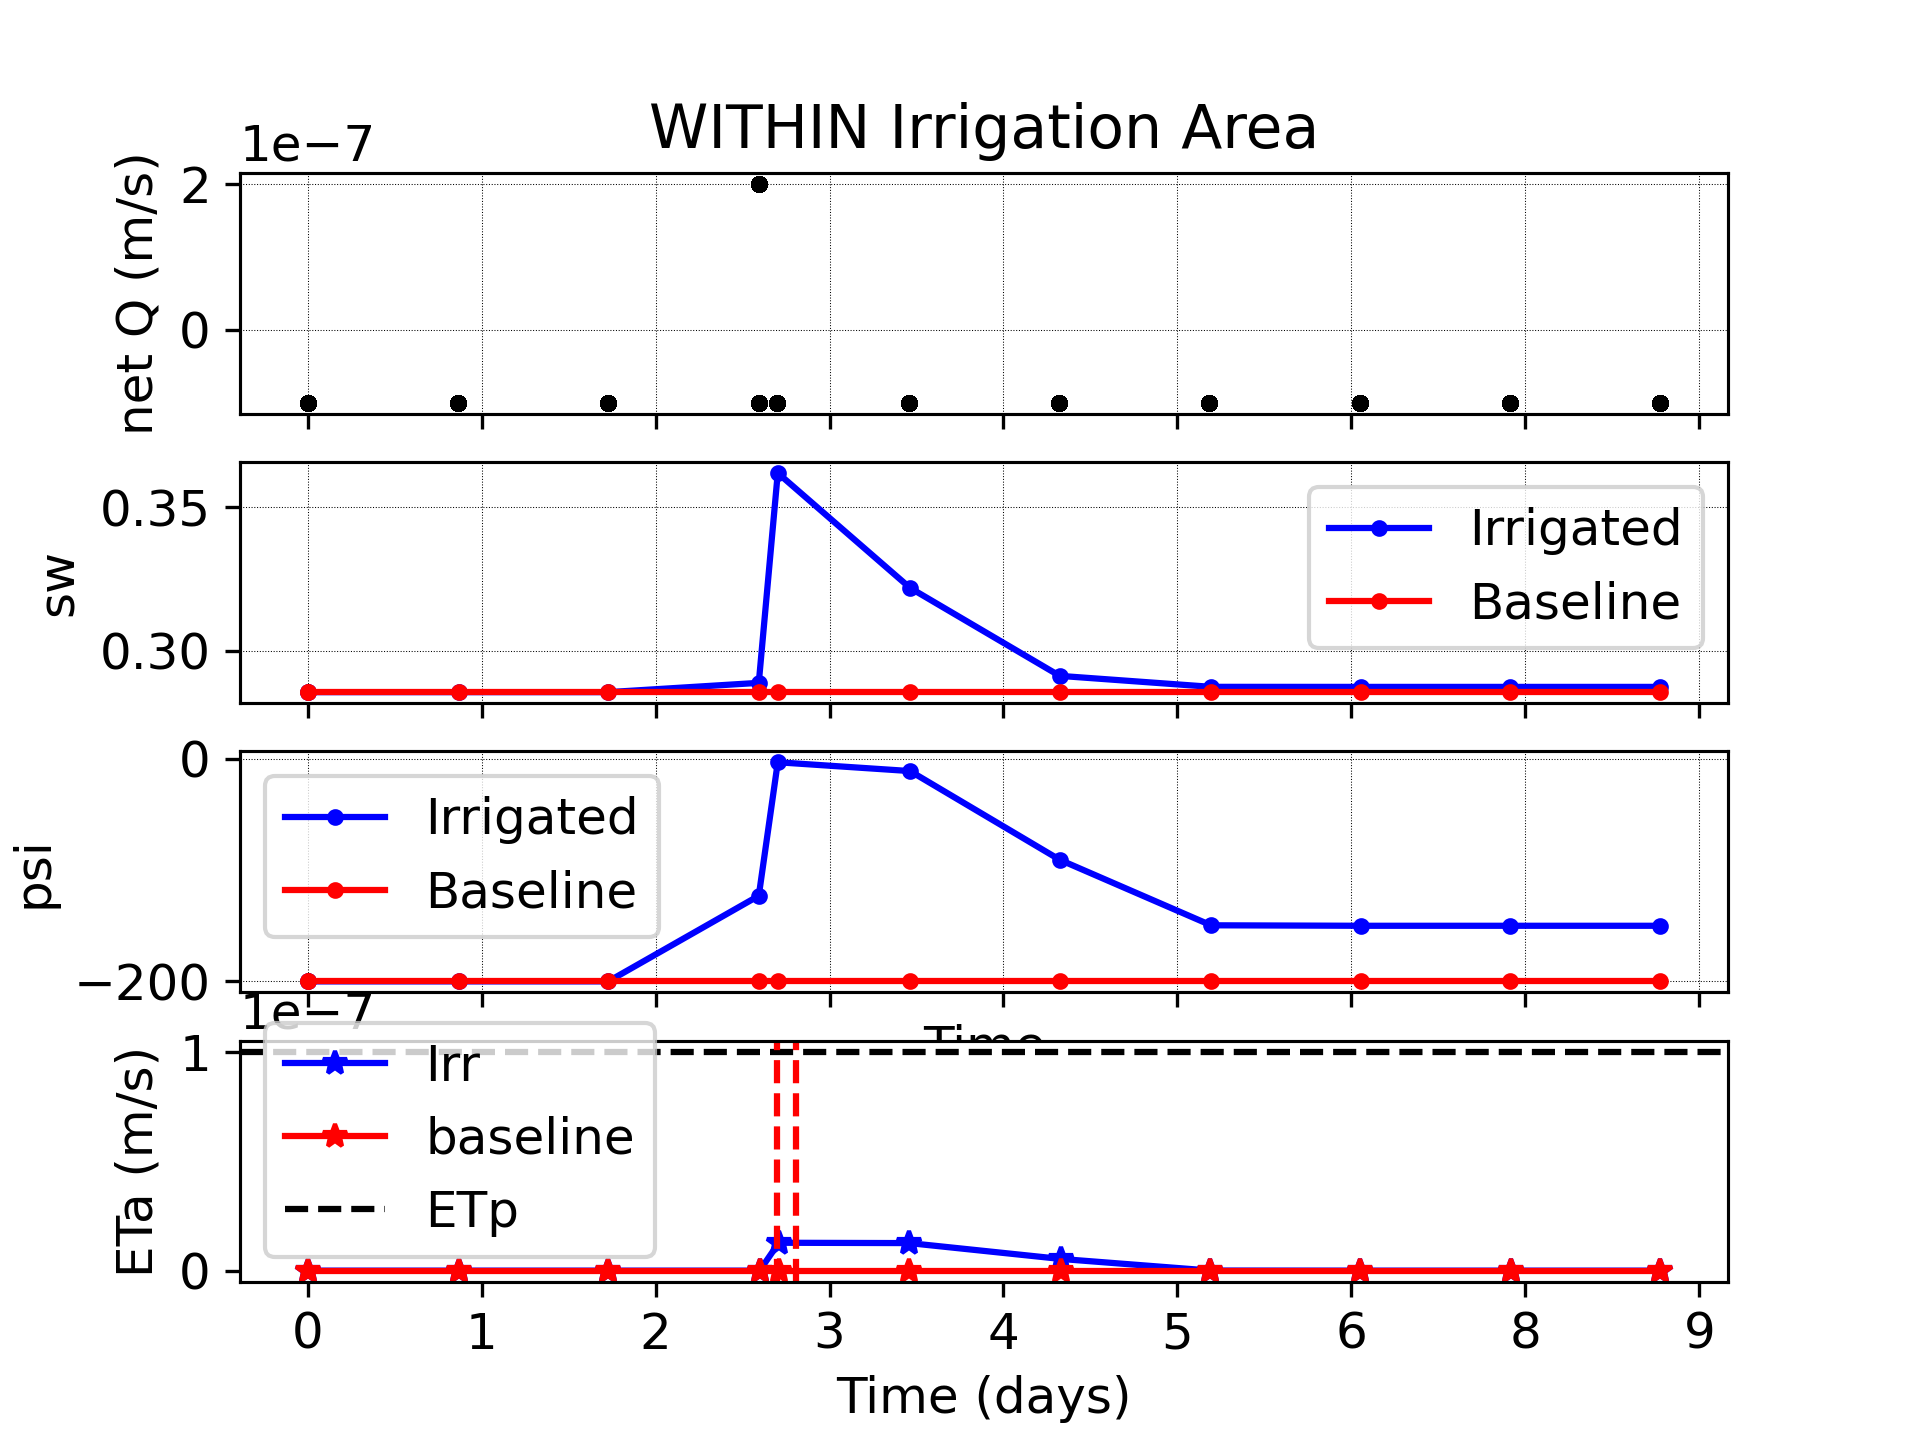
\includegraphics[width=0.875\linewidth]{files/plot_1d_evol_irrArea-4c0f10ad2fa8517ca684e5052156280c.png}
\caption*{Scenario 0, where irrigation triggering and length is highlighted by the dashad red vertical lines (approx. 3days). The plot show respectively the net atmospheric boundary conditions (ETp-Rain), the soil saturation water and pressure head on a surface node centered in the irrigation area. The bottom subplot shows the ETp (input), and the variation of ETa for both the baseline and with irrigation scheme.}
\end{figure}

\begin{figure}[!htbp]
\centering
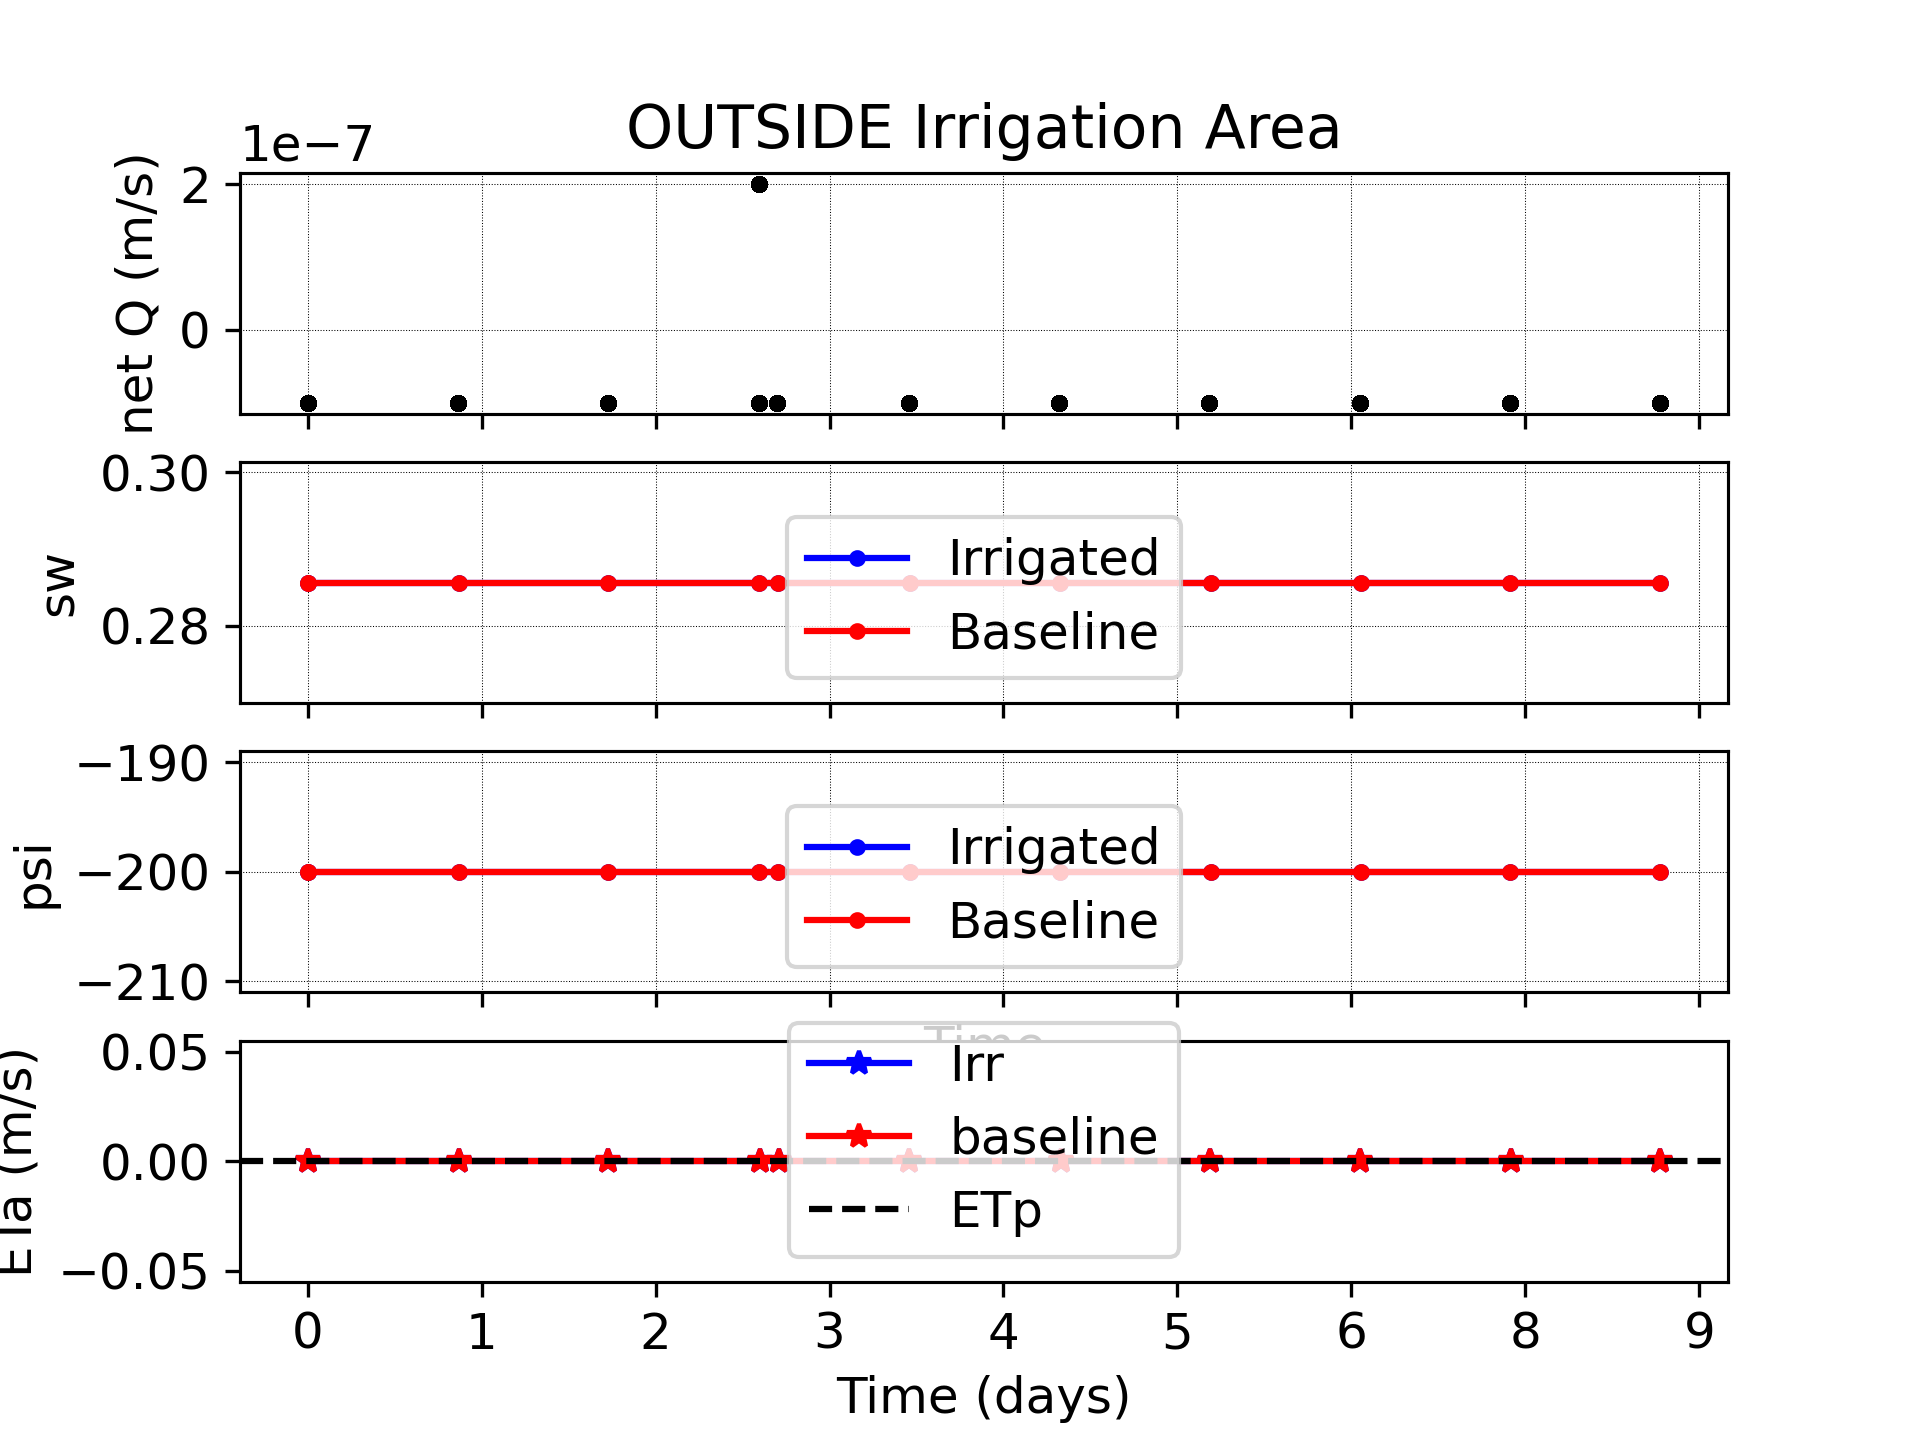
\includegraphics[width=0.875\linewidth]{files/plot_1d_evol_outArea-4651edee791016dd422d335828ba2785.png}
\caption*{SAME AS previous figure but outside the irrigation area.}
\end{figure}

\begin{figure}[!htbp]
\centering
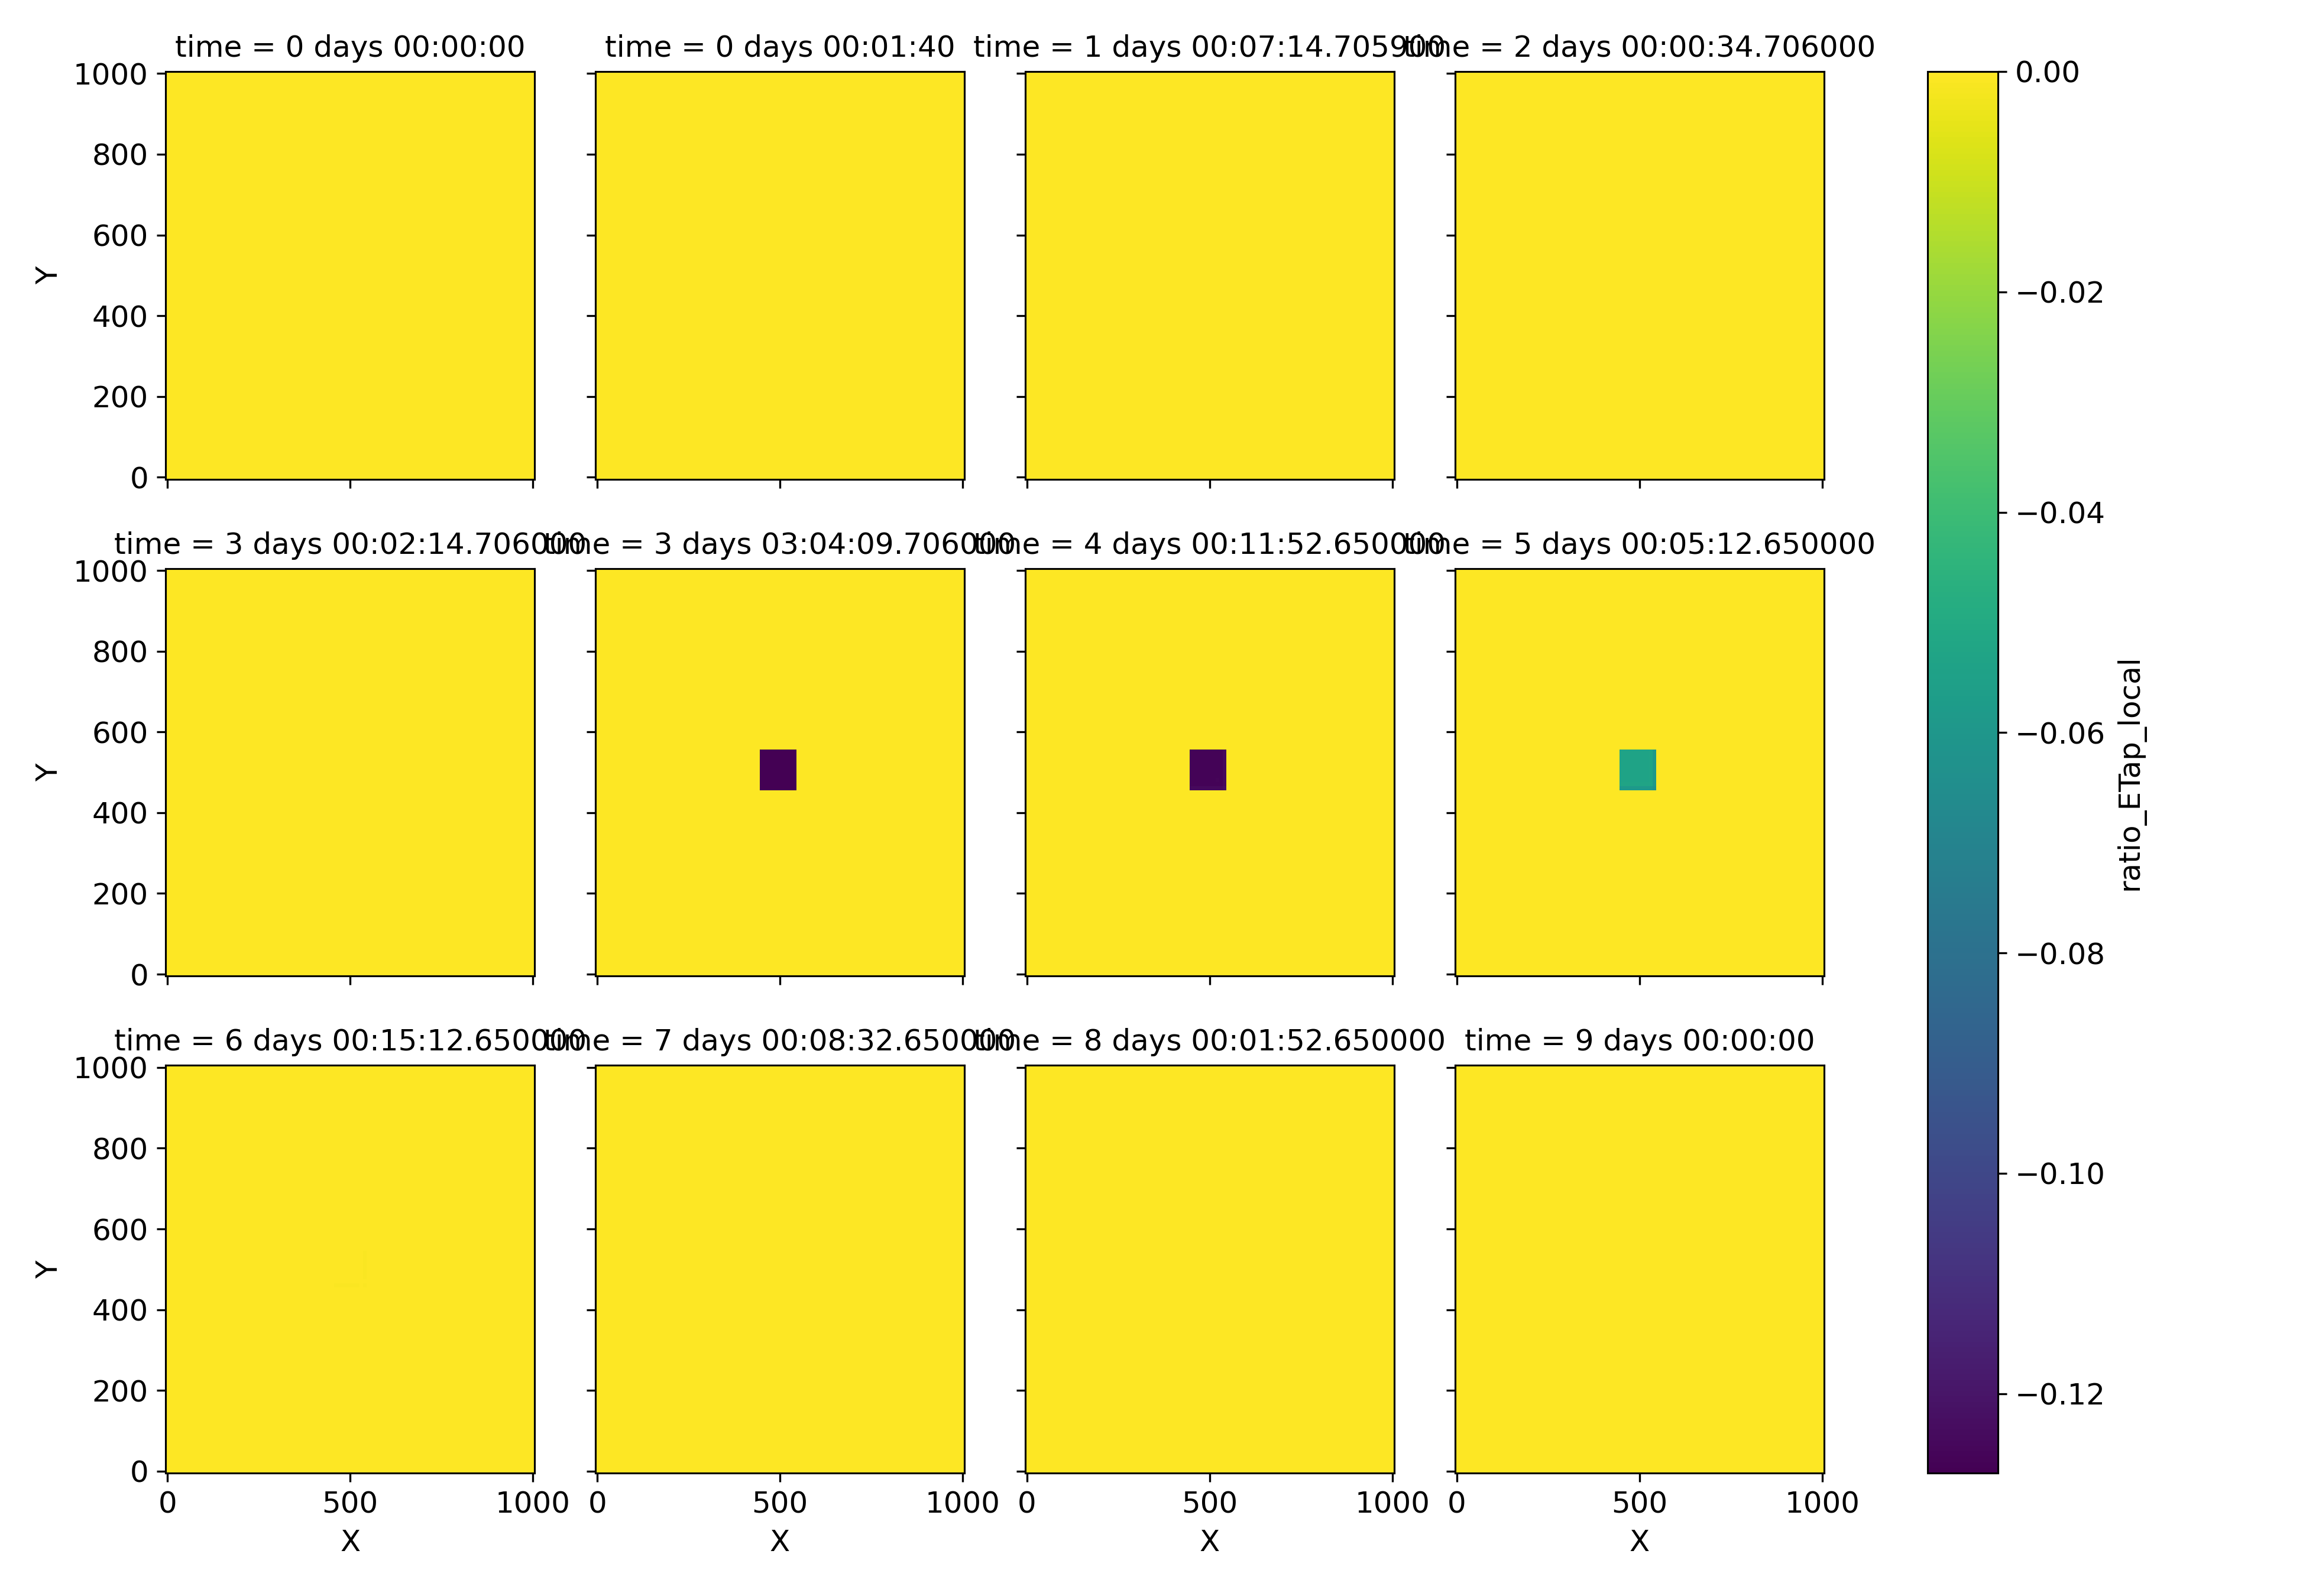
\includegraphics[width=0.875\linewidth]{files/ratioETap_withIRR_sp-49b67c2d818160e410a8535fe06acdc9.png}
\caption*{For each pixel we compute individually the ratio ETa/ETp.}
\end{figure}

\section{Irrigation accounting}

\begin{figure}[!htbp]
\centering
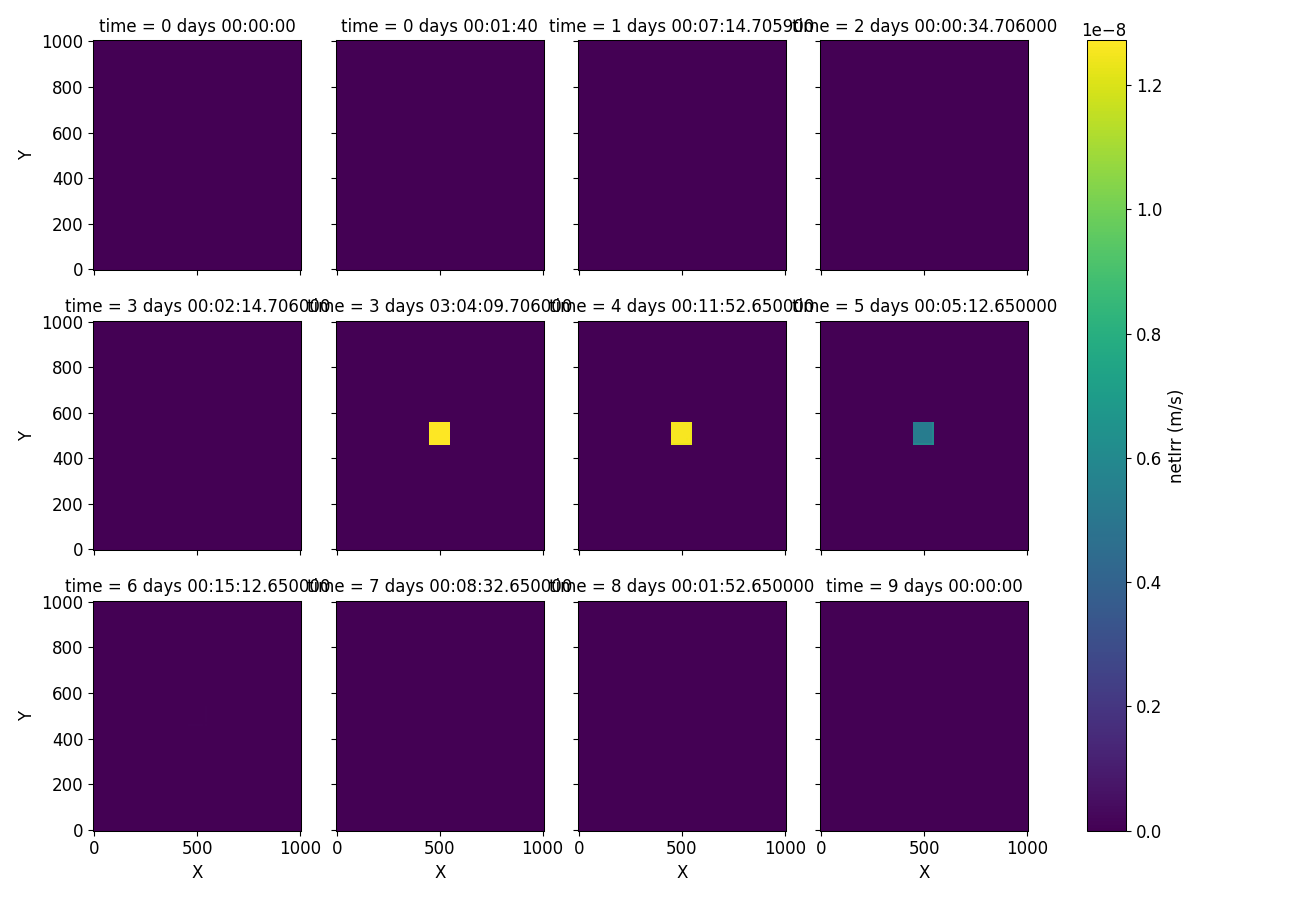
\includegraphics[width=0.875\linewidth]{files/netIrr_spatial_plot-3857eeb2205a5eeb9704563034b18cc5.png}
\caption*{netIrr\_spatial\_plot}
\end{figure}

\begin{figure}[!htbp]
\centering
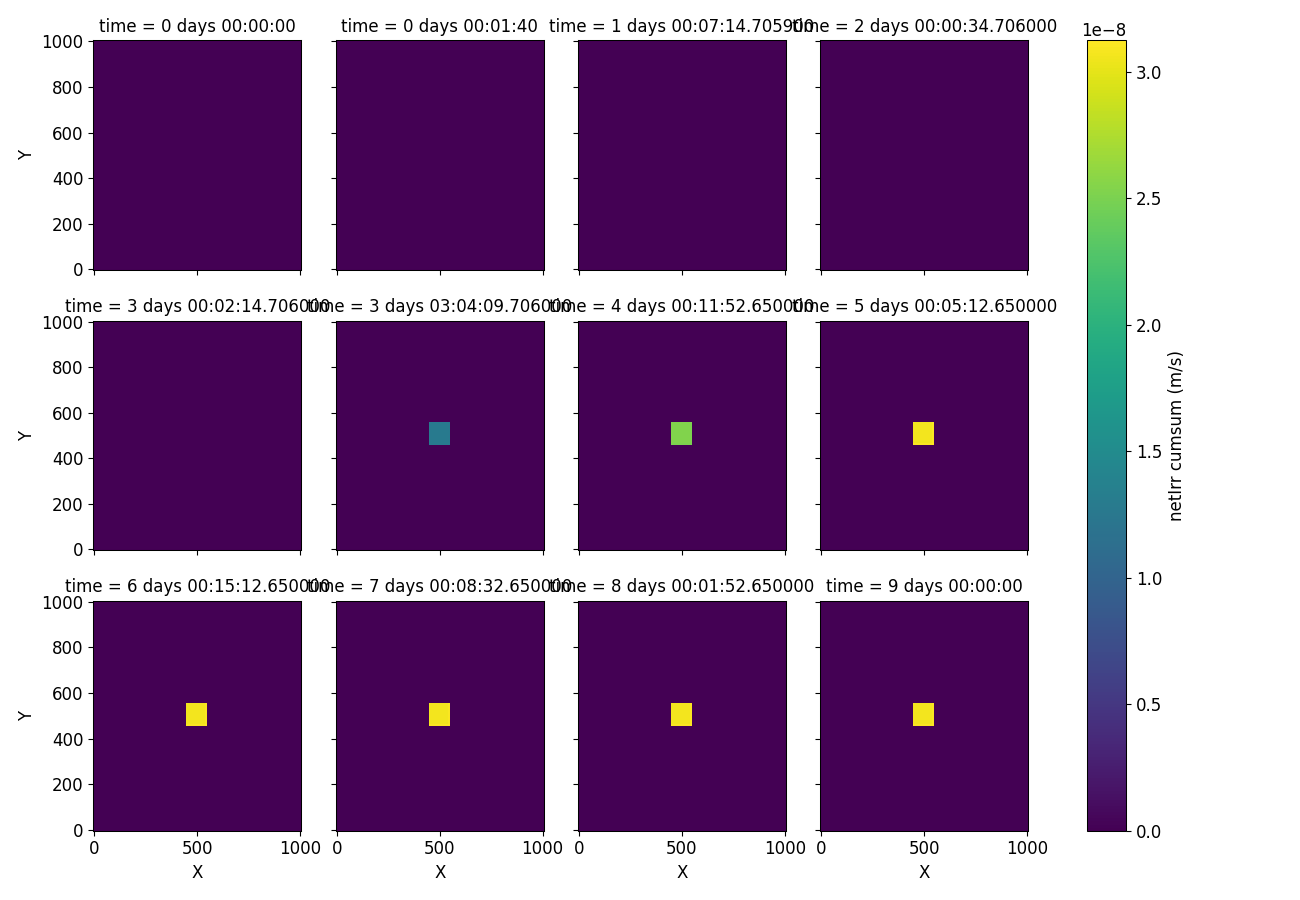
\includegraphics[width=0.875\linewidth]{files/netIrr_sumsum_spatia-d10967037bea75e5f728f0e00ebb3be5.png}
\caption*{netIrr\_sumsum\_spatial\_plot}
\end{figure}

\begin{figure}[!htbp]
\centering
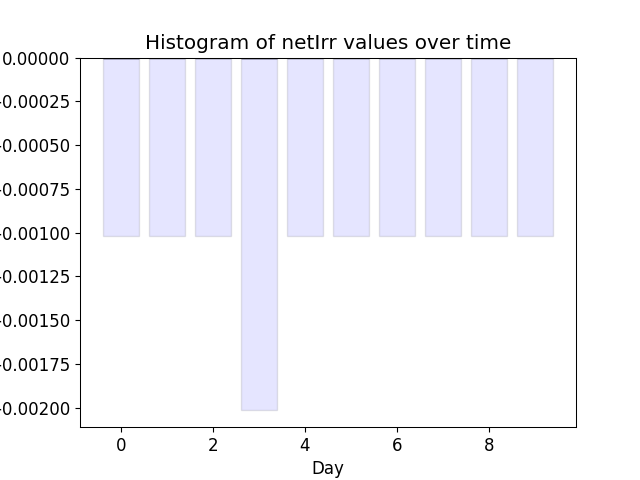
\includegraphics[width=0.875\linewidth]{files/bar_plot_netIrr-15bd447790e95df3852d4fed300027e3.png}
\caption*{bar\_plot\_netIrr}
\end{figure}

\section{Classification \& Decision}

The local and regional changes are then \textbf{compared to a number of thresholds} to try to detect if:

\begin{itemize}
\item a) There is no input of water into the soil (e.g. local ETa/p does not increase above a threshold)
\item b) There is input of water into the soil but due to rainfall (e.g. increase in regional ETa/p is over a
threshold and larger or similar to increase in local Eta/p)
\item c) There is input of water to the soil due to irrigation (e.g. increase in local ETa/p is over a
threshold and significantly larger than increase in regional ETa/p)
\end{itemize}

\begin{figure}[!htbp]
\centering
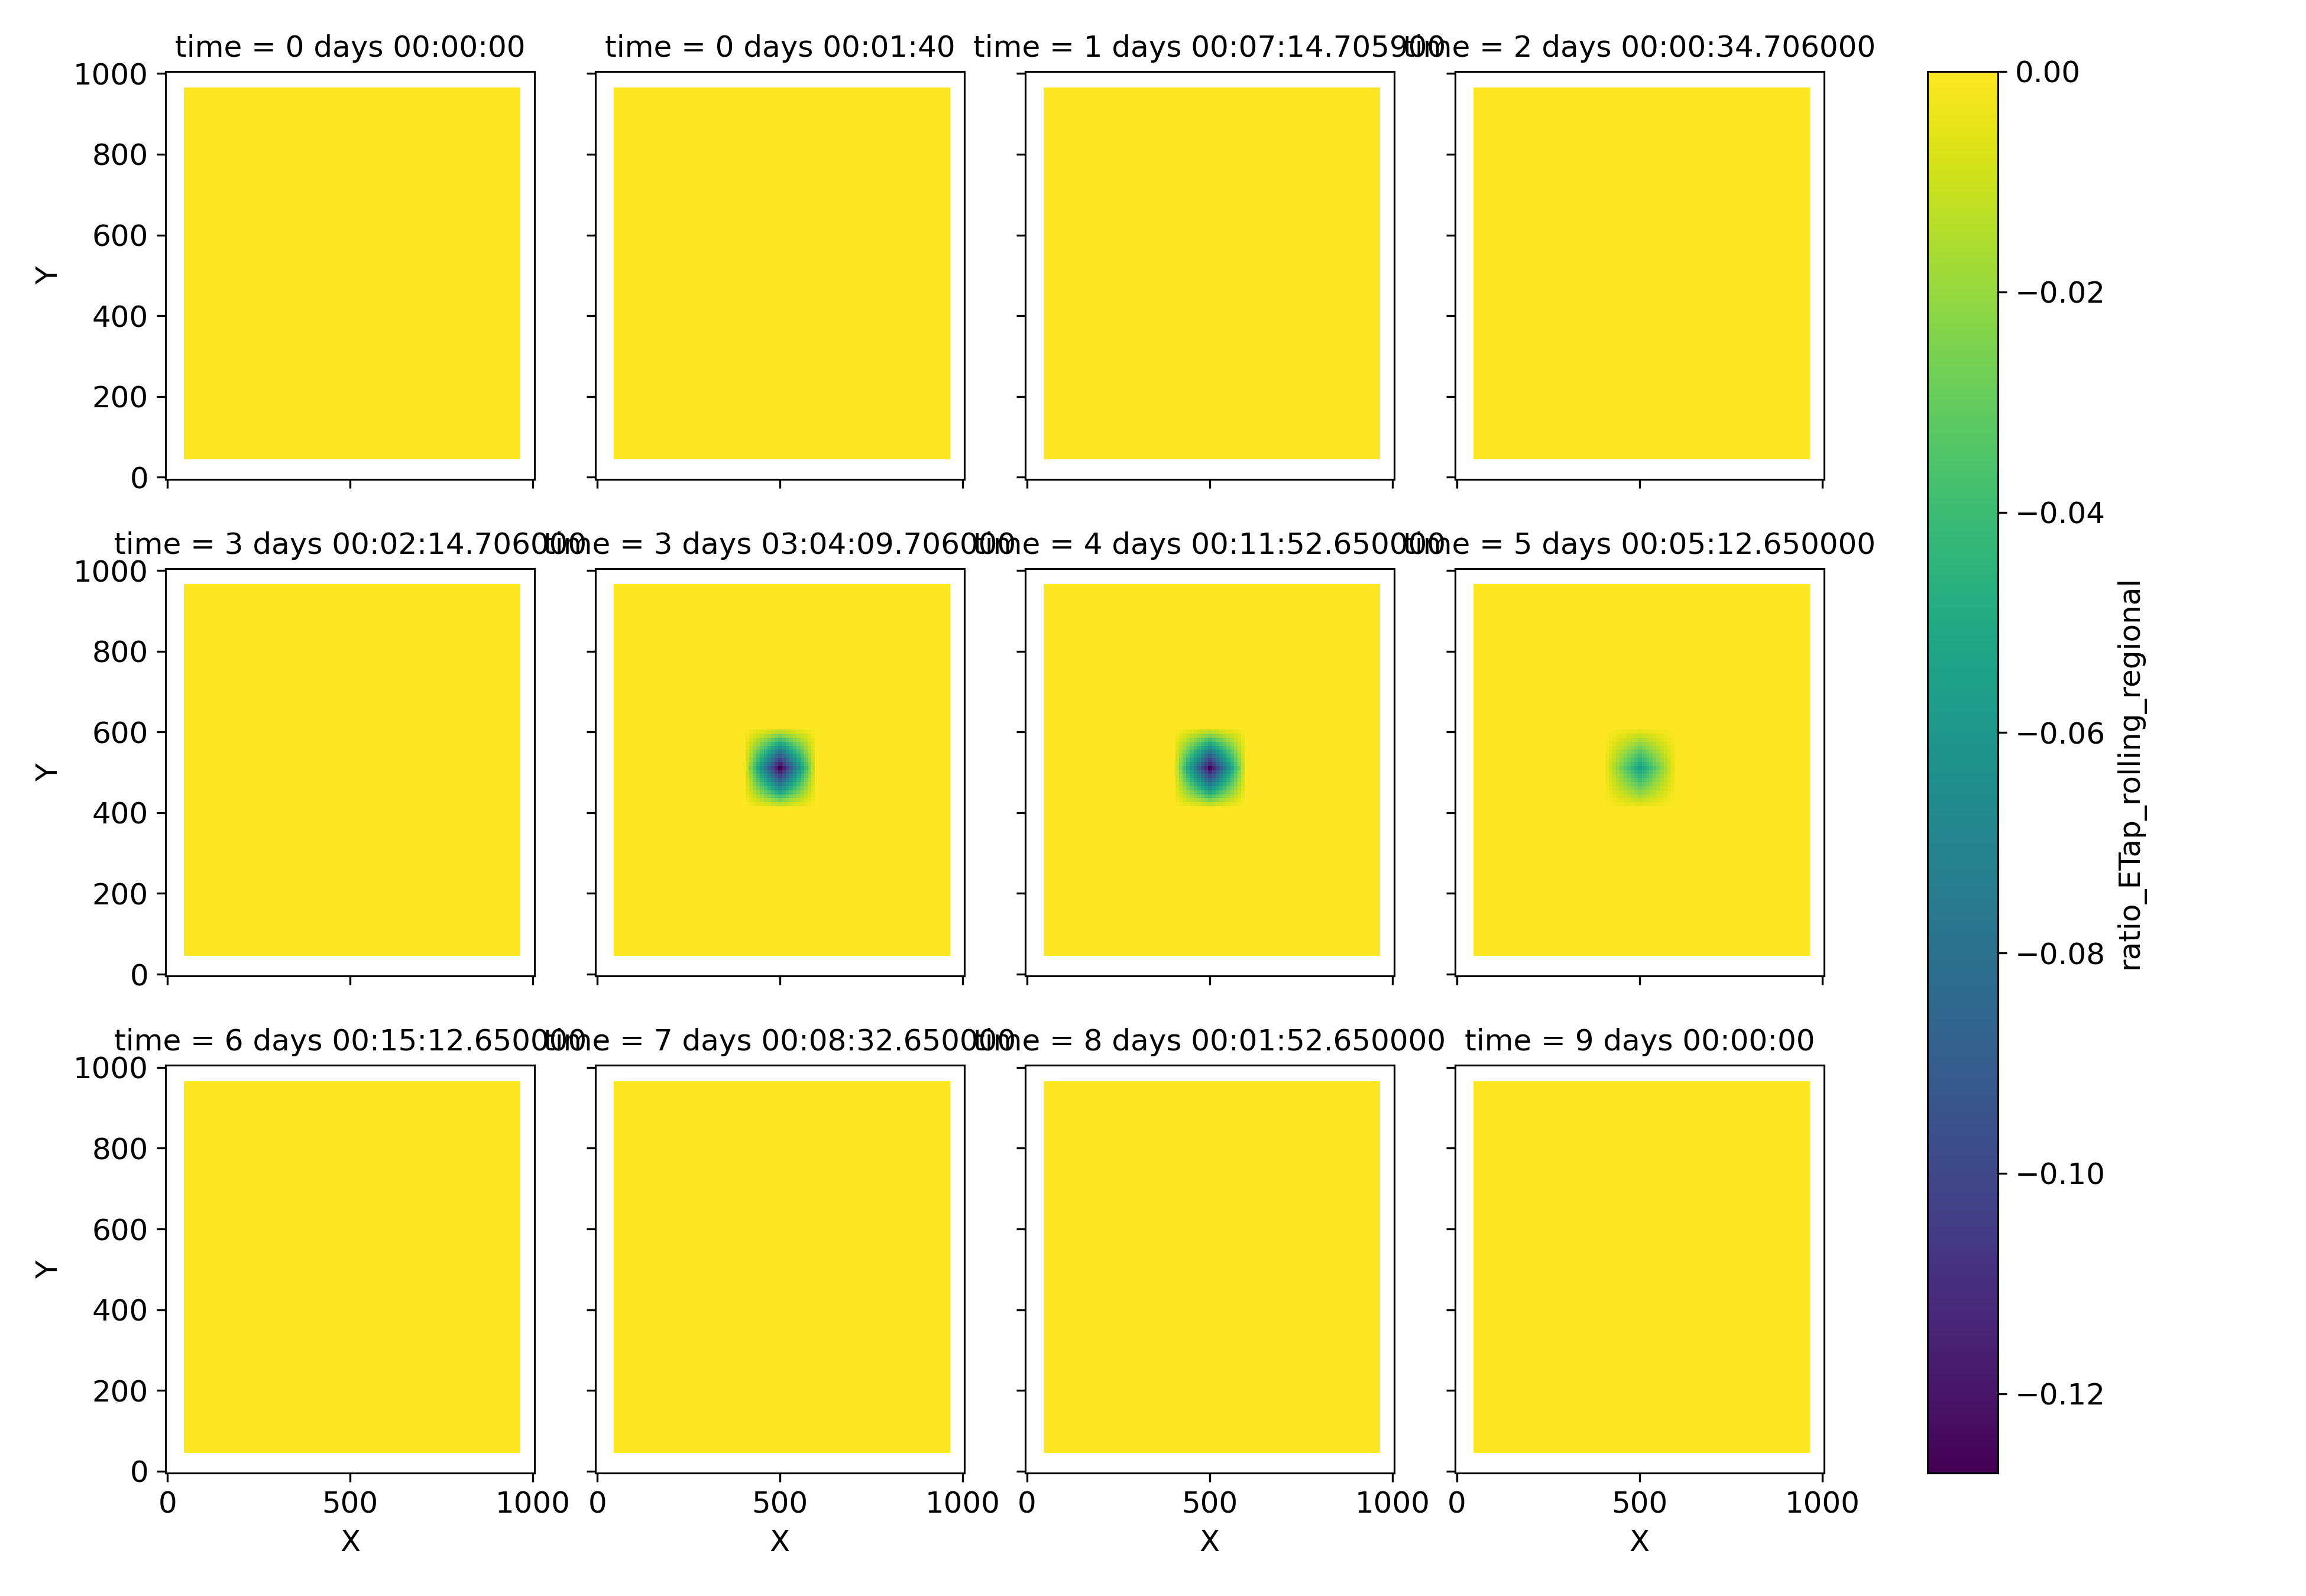
\includegraphics[width=0.875\linewidth]{files/ratioETap_regional_w-2c79d25fb6ed135ae56de174f4100705.png}
\caption*{There is input of water into the soil but due to rainfall : increase in regional ETa/p is over a
threshold and larger or similar to increase in local Eta/p)}
\end{figure}

\begin{figure}[!htbp]
\centering
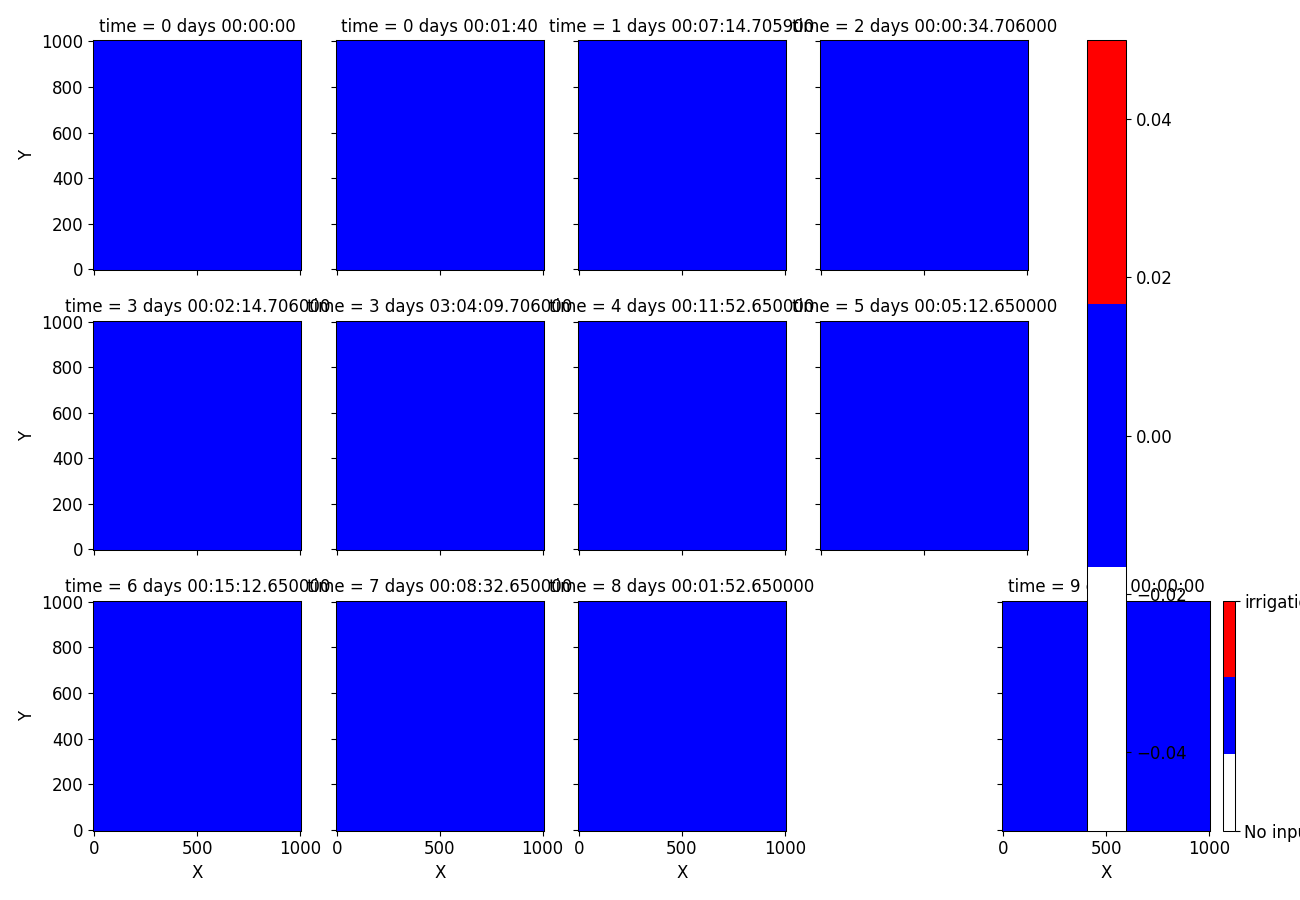
\includegraphics[width=0.875\linewidth]{files/classify_events-61db58665a3dabf47f3a3f60a5ac0fe0.png}
\caption*{classify\_events}
\end{figure}

\begin{figure}[!htbp]
\centering
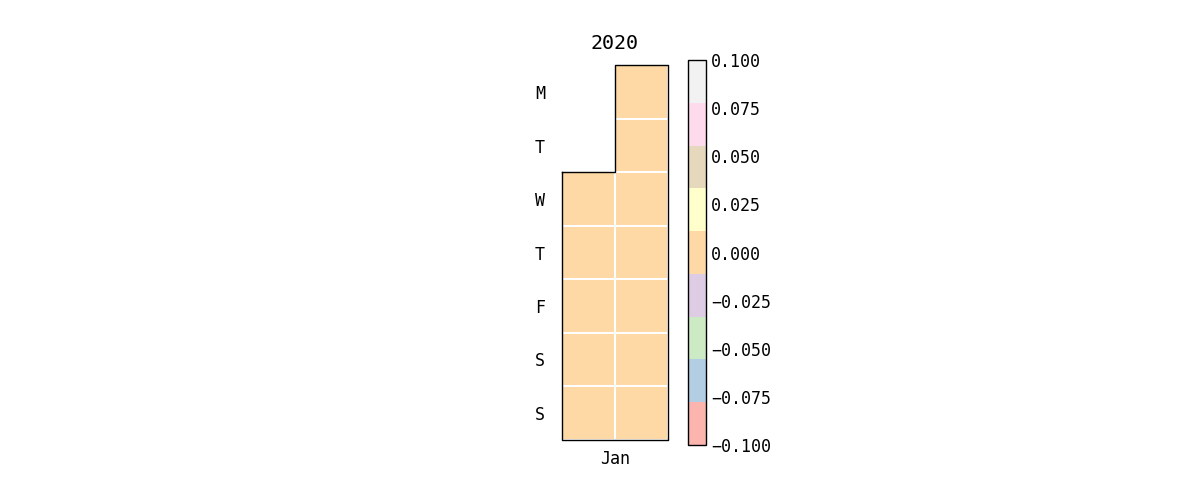
\includegraphics[width=0.01\linewidth]{files/events_calendar-1c52f0ad02e008e9966cfd99d8dda256.png}
\caption*{events\_calendar}
\end{figure}
\end{document}
